% =====================================================
\chapter{Style Transfer Baselines and Latent Optimisation Experiments}
\label{chap:csd_style}

% =====================================================
\section{Motivation}
\label{sec:ch7_motivation}

The experiments presented in the previous chapters have shown the effectiveness of diffusion-based atmospheric style transfer methods for generating visually realistic environmental transformations. Methods like StyleShot, CSGO, InstantStyle, and InstantStyle+ successfully transferred atmospheric properties like haze, fog, snow, and underwater look while preserving the semantic structure of the original scene. Qualitative evaluation revealed important changes in color distribution, contrast, illumination and overall mood, with outputs often closely resembling naturally occurring environmental conditions.

But even with these promising visual results, a deeper look into the generated images revealed a significant limitation. While the appearance of the images changed drastically, the semantic representations extracted by large-scale vision-language models often remained largely unchanged. Specifically, the CLIP-based assessment indicated that the generated images frequently maintained a high degree of consistency with the source-domain representations from which they were derived, despite the atmospheric change seeming visually plausible. This observation suggests that changes at the appearance level may not be enough to induce meaningful changes in the distribution of representations.

The distinction between visual realism and representation-level transformation is particularly relevant for robustness evaluation and domain adaptation. A generated image can appear very different to a human observer, but still be in a similar region of feature space when processed by modern vision-language models. Therefore, synthetic atmospheric generation methods that focus solely on visual realism may not be able to reproduce the semantic challenges faced in real-world environmental conditions.

Current approaches to atmospheric style transfer predominantly work with feed-forward conditioning mechanisms. The style reference image is fed into the diffusion model through attention-based conditioning modules, adapter networks or style injection mechanisms and the final image is generated through a single forward process of generation. But while these approaches allow efficient and controllable generation, they provide limited opportunity for iterative refinement once the sampling has started. During generation, the diffusion model is provided with a style signal, but it lacks a way to explicitly check that the generated image is still heading in the right direction towards the style distribution.

This limitation motivated the search for optimization-guided diffusion frameworks. The main idea is to treat style as an explicit optimization objective enforced throughout the reverse diffusion process, rather than a passive conditioning signal. In this formulation, the generated samples are continuously checked with respect to a target style representation and corrective updates are applied whenever the generated image diverges from the desired atmospheric characteristics.

Recent progress in constrained stable diffusion~\cite{zampini2025constrained} provides a natural foundation for this approach. The constrained diffusion framework formulates image generation as a constrained optimisation task within the denoising process itself, enabling generated samples to satisfy user-specified objectives without retraining the underlying diffusion model. Originally designed for material design optimisation and copyright-aware image generation, it provides an appealing mechanism for incorporating atmospheric style constraints into image synthesis.

This chapter investigates whether atmospheric style transfer can be formulated as a constrained optimisation problem in the reverse diffusion process. A spectrum of increasingly complex guidance strategies is explored, ranging from simple latent correction with Contrastive Style Descriptor (CSD~\cite{somepalli2024csd}) embeddings to perceptual guidance, frequency-aware constraints, Langevin dynamics, and proximal optimisation methods. The investigation aims to understand the effects of optimisation-based guidance on atmospheric style fidelity, content preservation, and controllability during diffusion-based image generation.

\begin{figure}[htbp]
    \centering
    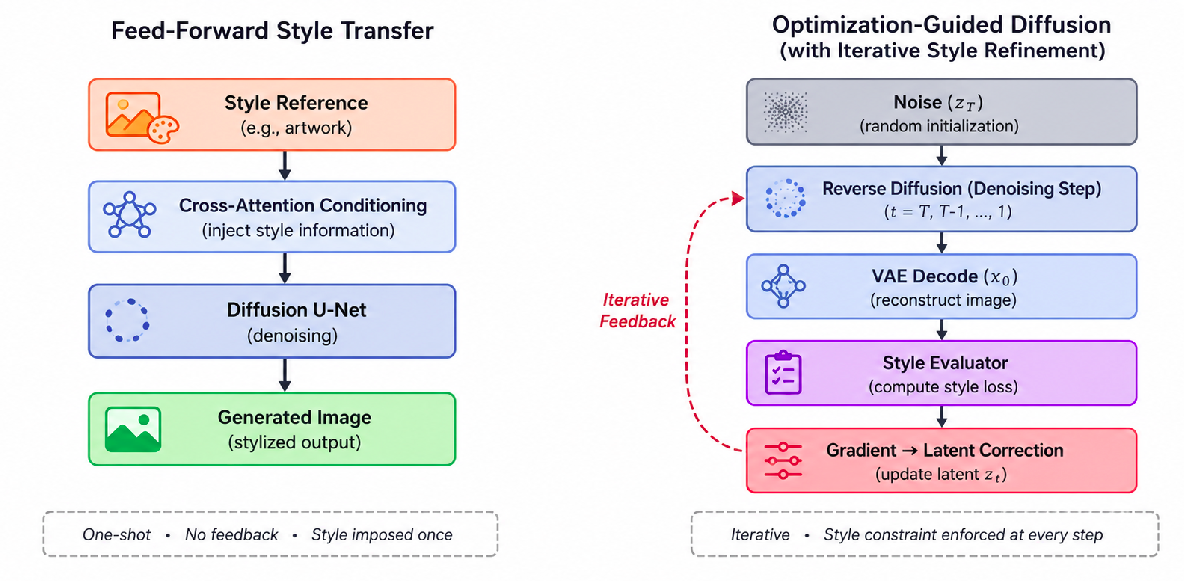
\includegraphics[width=0.95\linewidth]{images/figure_7.1.png}
    \caption{Conceptual comparison between the traditional feed-forward style transfer and the optimization-guided diffusion with iterative style refinement.}
    \label{fig:ch7_motivation}
\end{figure}

\FloatBarrier
% =====================================================
\section{Stable Diffusion with Constraints}
\label{sec:ch7_csd_theory}

Diffusion models have recently achieved remarkable success and become one of the most powerful frameworks for controllable image generation. Modern diffusion systems like Stable Diffusion~\cite{rombach2022ldm} and SDXL~\cite{podell2023sdxlimprovinglatentdiffusion} are able to produce very realistic images from text descriptions in an iterative denoising process over latent representations. While they have impressive capabilities, conventional diffusion models are inherently limited by the conditioning signals they have at inference. Once generation starts, the learned score function and the conditioning information provided mostly dictate the denoising trajectory, with little opportunity to impose external constraints.

Recent research has explored directly incorporating optimization objectives into the reverse diffusion process. These approaches, collectively known as constrained diffusion methods, aim to guide generated samples toward desired properties while preserving the generative capabilities of pretrained diffusion models. Diffusion is constrained by explicit objectives which are evaluated throughout the denoising process, not only via a prompt or reference image.

One of the most influential works in this direction is the constrained stable diffusion framework~\cite{zampini2025constrained}, which formulates image generation as a constrained optimisation problem. Instead of retraining model parameters, the framework operates fully at inference time by applying latent-space corrections defined by user-specified constraints. This formulation enables a pretrained diffusion model to meet external objectives without compromising generation quality or requiring extra supervision.

Let $z_t$ be the latent representation at diffusion timestep $t$. During normal diffusion sampling, the latent is evolved according to learned reverse diffusion dynamics. In the constrained setting, an additional objective function $g(x)$ is introduced, where
\begin{equation}
    x = D(z_t)
\end{equation}
denotes the decoded image from the frozen variational autoencoder (VAE) decoder $D(\cdot)$.

This constrained generation problem can be written as
\begin{equation}
    \min_x\; f(x) \quad \text{subject to} \quad g(x) \leq 0,
\end{equation}
where $f(x)$ is the diffusion objective and $g(x)$ is a user-specified constraint.

The main idea behind constrained diffusion is that generated samples can be periodically checked against the constraint function and corrected when violations occur. Instead of letting the denoising trajectory evolve naturally, optimization steps are introduced to guide latent representations to locations satisfying the desired constraints.

\begin{figure}[htbp]
    \centering
    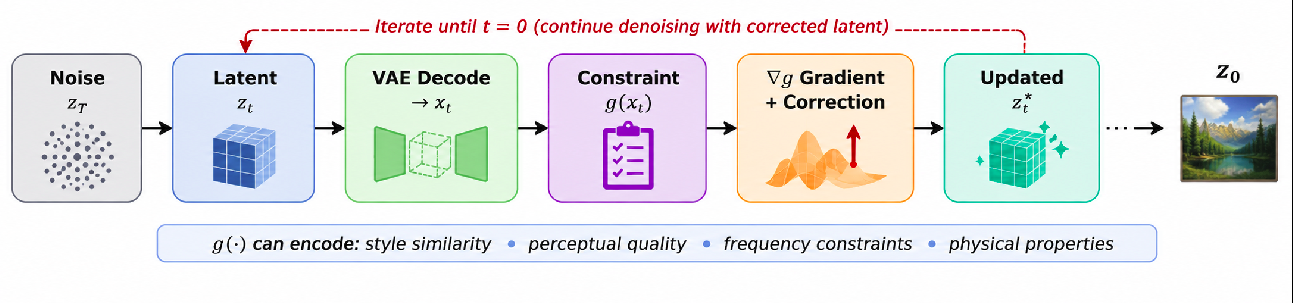
\includegraphics[width=0.95\linewidth]{images/figure_7.2.png}
    \caption{General constrained diffusion framework~\cite{zampini2025constrained}. Latent representations are decoded periodically, evaluated against a constraint function, and corrected before the denoising process continues.}
    \label{fig:ch7_csd_framework}
\end{figure}

One of the important advantages of this framework is flexibility. The constraint function can encode a wide class of objectives such as semantic similarity, style consistency, perceptual quality, physical properties, geometric constraints or task-specific requirements. Hence, constrained diffusion is a generic mechanism to inject external knowledge into image generation without modifying the pre-trained diffusion model itself.

An important benefit is the separation of generation and optimization. The constraint function guides the task, while the diffusion model is still responsible for generating realistic images. This modular design allows for the addition of new objectives without retraining the generative backbone and enables rapid experimentation with alternative constraint formulations.

Constrained diffusion provides an attractive alternative to traditional feed-forward conditioning in the setting of atmospheric style transfer. Instead of injecting style information solely via cross-attention mechanisms, atmospheric features can be modelled as optimisation objectives applied throughout the reverse diffusion process. This formulation enables continuous refinement of generated images and provides direct control over the evolution of atmospheric appearance during sampling.

\FloatBarrier
% =====================================================
\section{Style Guidance with Contrastive Style Descriptors}
\label{sec:ch7_csd_guidance}

The constrained diffusion framework outlined above provides a mechanism to incorporate arbitrary objectives into the reverse diffusion process. But the quality of the resulting guidance critically depends on the choice of constraint function. For atmospheric style transfer, an appropriate constraint is needed that captures visual properties associated with environmental phenomena but is robust to variations in scene content, object arrangement and semantic structure.

Existing style transfer approaches generally employ either low-level texture statistics or feature correlations obtained from convolutional neural networks. While such representations are suitable for artistic style transfer, they usually do not account for higher-level atmospheric properties like visibility degradation, color attenuation, illumination changes and the overall environmental appearance. Furthermore, these representations are often very sensitive to scene content, and thus not suitable for atmospheric style guidance where content preservation is desired.

To address these limitations, this work explores the use of Contrastive Style Descriptors (CSD)~\cite{somepalli2024csd} as a style-aware guidance mechanism. CSD is built on large-scale vision-language representations and is designed to separate style from semantic content. CSD learns a style representation that is consistent across different scenes with similar visual characteristics, unlike traditional feature extractors that mix object identity and appearance.

For a generated image $x_g$ and a reference style image $x_s$, the CSD encoder generates style embeddings as follows:
\begin{equation}
    s_g = S(x_g), \qquad s_s = S(x_s),
\end{equation}
where $S(\cdot)$ is the frozen style encoder.

The similarity between the generated style and the reference style is calculated by cosine similarity:
\begin{equation}
    \mathrm{Sim}(s_g, s_s) = \frac{s_g \cdot s_s}{\|s_g\|\,\|s_s\|}.
\end{equation}

A style loss can then be defined as:
\begin{equation}
    L_{\text{style}} = 1 - \mathrm{Sim}(s_g, s_s).
\end{equation}

Minimizing this objective encourages the generated images to be close to the target atmospheric style manifold while preserving the semantic information inherited from the diffusion model.

The proposed guidance mechanism is illustrated in Figure~\ref{fig:ch7_csd_guidance}. The latent representation is decoded into image space at selected diffusion timesteps, and passed through the frozen CSD encoder. The resulting style embedding is then compared to a reference atmospheric image and the resulting loss is backpropagated through the decoder to obtain gradients with respect to the latent representation. These gradients are then applied to improve the latent code before the denoising continues.

\begin{figure}[htbp]
    \centering
    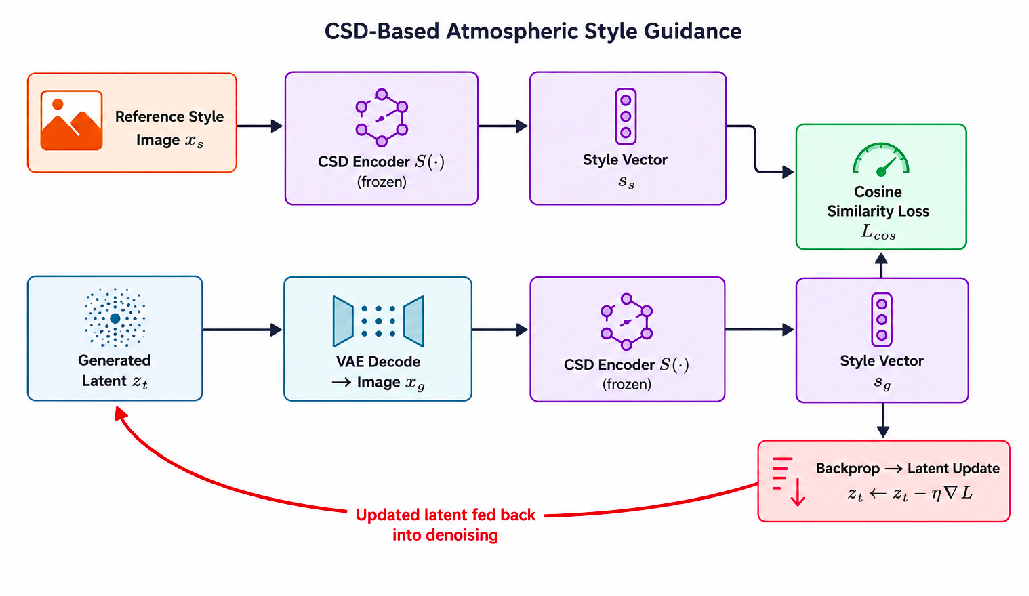
\includegraphics[width=0.95\linewidth]{images/figure_7.3.png}
    \caption{CSD-based atmospheric style guidance. Generated images are decoded from the latent representation, encoded by the frozen CSD network, and compared to a reference atmospheric style image.}
    \label{fig:ch7_csd_guidance}
\end{figure}

The main motivation for the use of CSD is the observation that the appearance statistics of atmospheric phenomena are often of a global nature rather than local texture patterns. Dense fog, haze, snowfall, underwater environments and sandstorms display distinct distributions of colour, contrast and visibility across the entire image. This means that the style embeddings learned with contrastive objectives are a better representation of atmospheric appearance than traditional texture-based descriptors.

The first hypothesis was that style similarity optimization in the CSD embedding space could enable direct control over the atmospheric look while maintaining content fidelity. If successful, the approach would provide a way of enforcing stylistic constraints over the reverse diffusion process, rather than relying only on feed-forward conditioning.

To test this hypothesis, a series of experiments was performed in which style losses based on CSD embeddings were included in the latent denoising process. The following section presents how these style objectives were propagated into the diffusion trajectory via gradient-based latent optimisation.

\begin{table}[htbp]
\centering
\caption{Initial CSD-guided diffusion configurations explored during atmospheric style transfer experiments.}
\label{tab:initial_csd}
\renewcommand{\arraystretch}{1.3}
\begin{tabular}{lll}
\toprule
\textbf{Experiment} & \textbf{Backbone} & \textbf{Guidance Objective} \\
\midrule
E1 & Stable Diffusion 1.5 & Cosine Similarity \\
E2 & Stable Diffusion 1.5 + LoRA & Cosine Similarity \\
E3 & SDXL & Cosine Similarity \\
E4 & SDXL & Cosine + Perceptual Loss \\
\bottomrule
\end{tabular}
\end{table}

\begin{figure}[htbp]
    \centering
    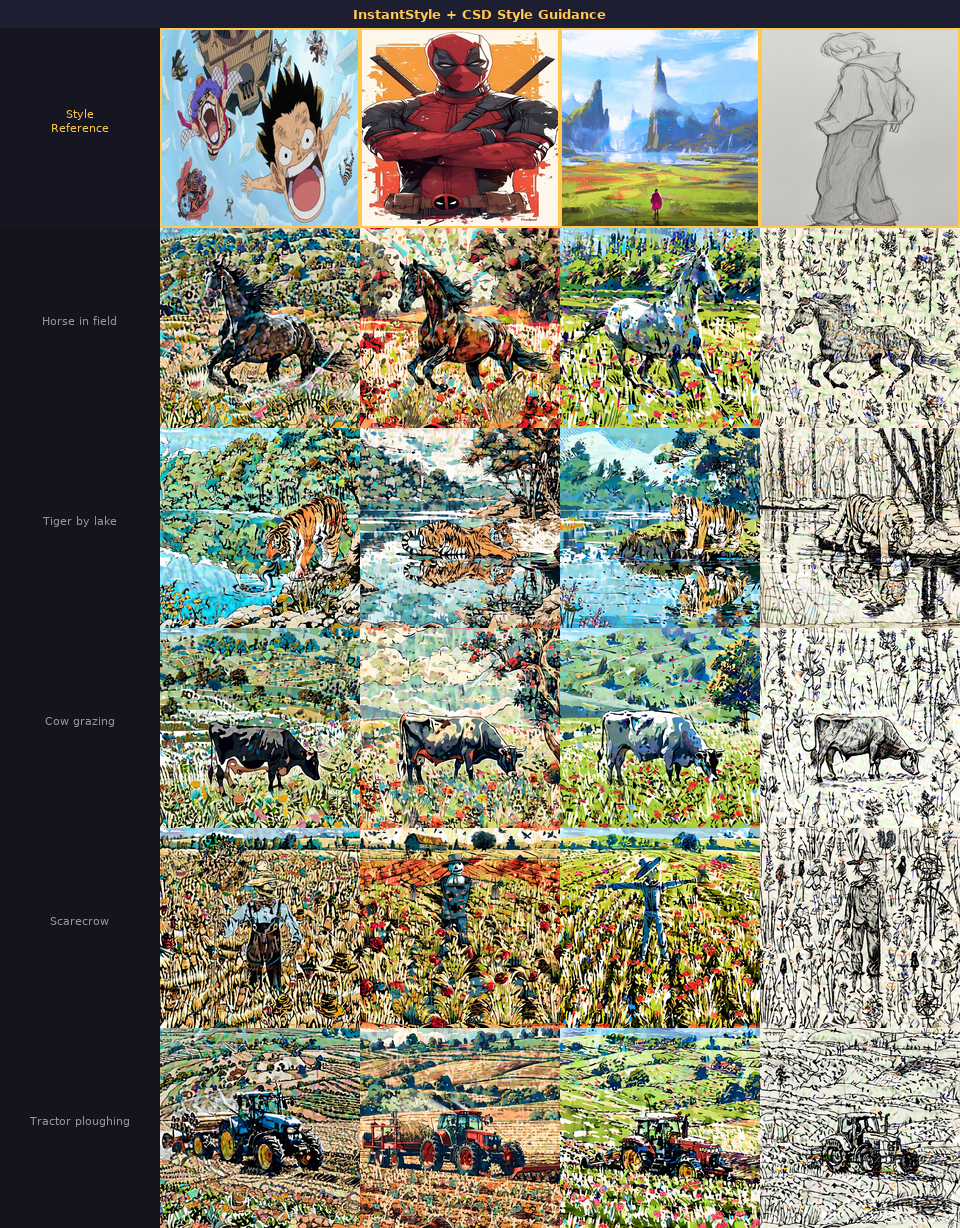
\includegraphics[width=0.88\linewidth, height=0.82\textheight, keepaspectratio]{images/ch7_grid_is_csd.png}
    \caption{InstantStyle + CSD guidance generation grid (seed 42). The first row shows the style reference image used as the guidance target for each atmospheric domain; subsequent rows show generated outputs for each content prompt. CSD guidance visibly shifts global appearance towards the target atmospheric domain, though aggressive gradient updates can introduce structural artefacts in complex scenes.}
    \label{fig:ch7_grid_is_csd}
\end{figure}

\FloatBarrier
% =====================================================
\section{Optimization in the Reverse Diffusion Process}
\label{sec:ch7_latent_opt}

The style constraint defined in the previous section provides a quantitative measure of the similarity between the atmospheric effect of a generated image and that of a reference style image. Having a suitable objective, however, is not sufficient on its own. To influence the generation process, the style loss must be backpropagated through the diffusion trajectory to modify the evolving latent representation.

Traditional diffusion sampling follows a fixed denoising path determined by the learned score function. At each time step, the model predicts a denoised prediction of the current latent representation, turning random noise step by step into a coherent image. In standard sampling, this process proceeds without any explicit feedback about whether the generated image is approaching the desired atmospheric style.

The main idea investigated in this work is to halt denoising at certain points in time and perform style-aware latent refinement. Instead of letting the latent representation evolve freely, the intermediate samples are decoded and evaluated through the CSD style encoder and corrected via gradient-based optimization.

Let $z_t$ be the latent representation at the diffusion step $t$. The latent is first decoded to image space using the frozen variational autoencoder:
\begin{equation}
    x_t = D(z_t),
\end{equation}
where $D(\cdot)$ denotes the VAE decoder.

The generated image is then fed into the CSD encoder to calculate the style loss:
\begin{equation}
    L_{\text{style}} = 1 - \cos\!\bigl(S(x_t),\; S(x_s)\bigr),
\end{equation}
where $x_s$ is the reference atmospheric style image.

Gradients are then calculated with respect to the latent representation:
\begin{equation}
    g_t = \nabla_{z_t} L_{\text{style}}.
\end{equation}

These gradients are used to perform a latent correction step:
\begin{equation}
    z_t' = z_t - \eta\, g_t,
\end{equation}
where $\eta$ is the learning rate for guidance.

The corrected latent representation is then fed back into the diffusion process and the denoising is continued normally until the next optimization step. This procedure is applied iteratively to steer the generated image toward the target atmospheric style manifold, while preserving the semantic structure inherited from the pretrained diffusion model.

\begin{figure}[htbp]
    \centering
    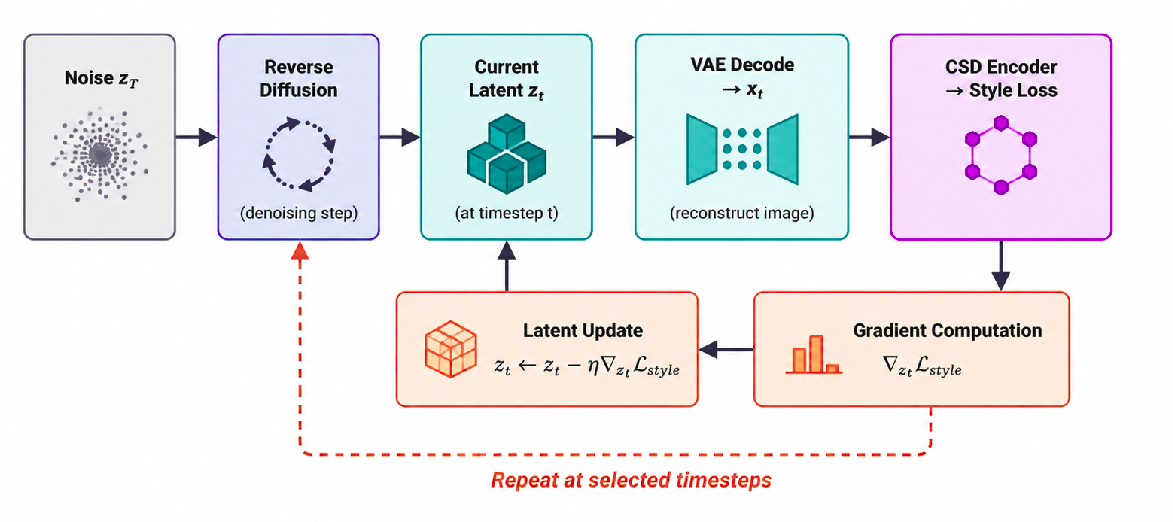
\includegraphics[width=0.95\linewidth]{images/figure_7.5.png}
    \caption{Optimization-guided refinement of latent representations. At selected timesteps the latent is decoded, evaluated by the style loss, corrected via gradient updates, and fed back into denoising.}
    \label{fig:ch7_latent_opt}
\end{figure}

One key design decision is the frequency of optimisation updates. Correcting at each denoising step adds large computational overhead and can destabilise the diffusion trajectory. Infrequent updates, however, may provide insufficient guidance to steer the final image. A range of update schedules was investigated, from dense optimisation throughout the full denoising process to sparse corrections applied only at later generation stages.

Another important factor is the scale of the guidance signal. Excessively large latent corrections can overpower the diffusion prior, leading to unrealistic images, semantic distortions, or collapse toward the reference style image. Very small updates, conversely, do not produce meaningful atmospheric transformations. Balancing generation fidelity and style adherence therefore emerged as one of the central challenges of optimisation-guided diffusion.

Initial experiments confirmed that simple latent correction can influence global image appearance and improve similarity with the target style distribution. The behaviour obtained, however, depends strongly on the choice of optimisation hyperparameters, guidance schedules, and diffusion backbone. Aggressive optimisation frequently produced unrealistic visual results or destroyed important semantic information present in the original scene.

These observations motivated further investigation into the relationship between guidance strength and content preservation. Experiments with different optimisation schedules showed that the timing of style corrections is critical for output quality. The following section examines this relationship via Langevin dynamics and stochastic latent refinement.

\begin{table}[htbp]
\centering
\caption{Optimization parameters explored during latent refinement experiments.}
\label{tab:latent_optimization}
\renewcommand{\arraystretch}{1.3}
\begin{tabular}{lll}
\toprule
\textbf{Parameter} & \textbf{Values Tested} & \textbf{Reason} \\
\midrule
Learning rate & 0.001 -- 0.1 & Control update magnitude \\
Guidance Frequency & Sparse / Dense & Update scheduling \\
Optimization Steps & 1 -- 10 & Correction strength \\
Diffusion Backbone & SD1.5 / SDXL & Model comparison \\
Style Objective & Cosine Similarity & Atmospheric alignment \\
\bottomrule
\end{tabular}
\end{table}

\FloatBarrier
% =====================================================
\section{Langevin Dynamics for Latent Refinement}
\label{sec:ch7_langevin}

The previous section describes a gradient-based optimization strategy that showed that the atmospheric style characteristics can be manipulated with a latent correction strategy. However, the updates generated were entirely deterministic and frequently behaved unstably. In several experiments, strong style gradients caused a significant deviation of the optimization process from the natural diffusion trajectory, leading to distorted structures, unrealistic textures and severe semantic degradation.

This observation led us to explore stochastic optimization techniques that can balance style guidance with the inherent generative prior of the diffusion model. Among the approaches available, Langevin Dynamics is especially attractive, as it combines gradient-based optimization with controlled stochastic exploration.

Langevin Dynamics is a technique developed for Bayesian inference and sampling from complex probability distributions. It adds Gaussian noise to the deterministic gradient updates. This additional stochastic term allows samples to explore nearby regions of the latent space while still moving towards regions that satisfy the desired objective.

The Langevin update for a latent representation $z_t$ can be written as:
\begin{equation}
    z_{t+1} = z_t - \eta\,\nabla_z L(z_t) + \sqrt{2\eta}\,\epsilon_t,
\end{equation}
where $\eta$ is the optimization step size, $L(z_t)$ is the style objective, and $\epsilon_t \sim \mathcal{N}(0, I)$ is Gaussian noise.

The extra stochastic term serves two important purposes over the deterministic latent correction strategy introduced above. First, it keeps optimization from getting stuck in bad local minima. Second, it maintains sample diversity by ensuring that the latent trajectories keep exploring reasonable regions of the diffusion manifold.

\begin{figure}[htbp]
    \centering
    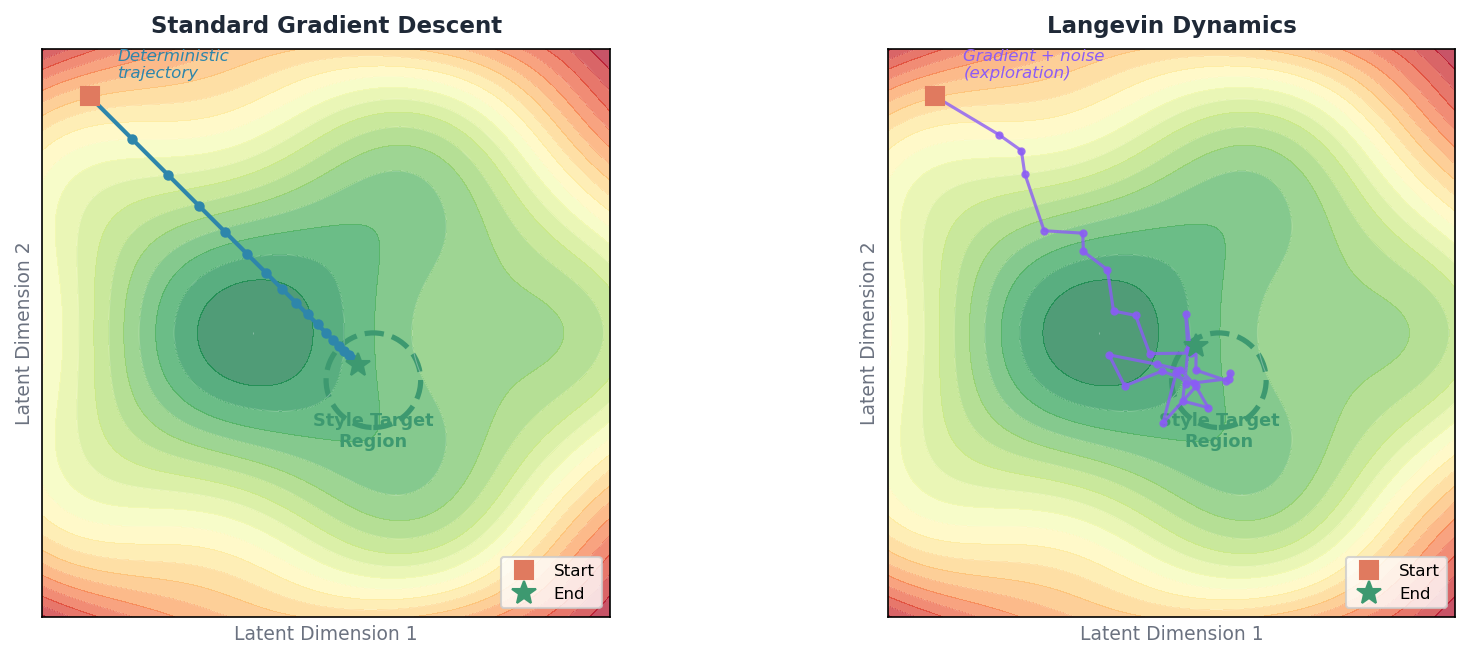
\includegraphics[width=0.95\linewidth]{images/ch7_langevin_concept.png}
    \caption{Conceptual depiction of the Langevin-based latent refinement. The latent representation is optimized toward high style similarity while preserving stochastic exploration of the diffusion manifold.}
    \label{fig:ch7_langevin_concept}
\end{figure}

A set of experiments was performed, using Langevin refinement at different stages of the denoising process. In the first experiments the optimization updates were applied along the entire reverse diffusion trajectory. While this approach resulted in higher style similarity scores, the generated images often suffered from severe semantic distortions. Foreground objects were partially corrupted, structural details were lost and in extreme cases the generated image began to look more like the reference style image than the original content.

Representative failure cases encountered in early experiments are illustrated in Figure~\ref{fig:ch7_langevin_failure}. Strong optimization caused the latent representation to deviate from the natural diffusion path, resulting in unnatural image formation and reduced content preservation.

\begin{figure}[htbp]
    \centering
    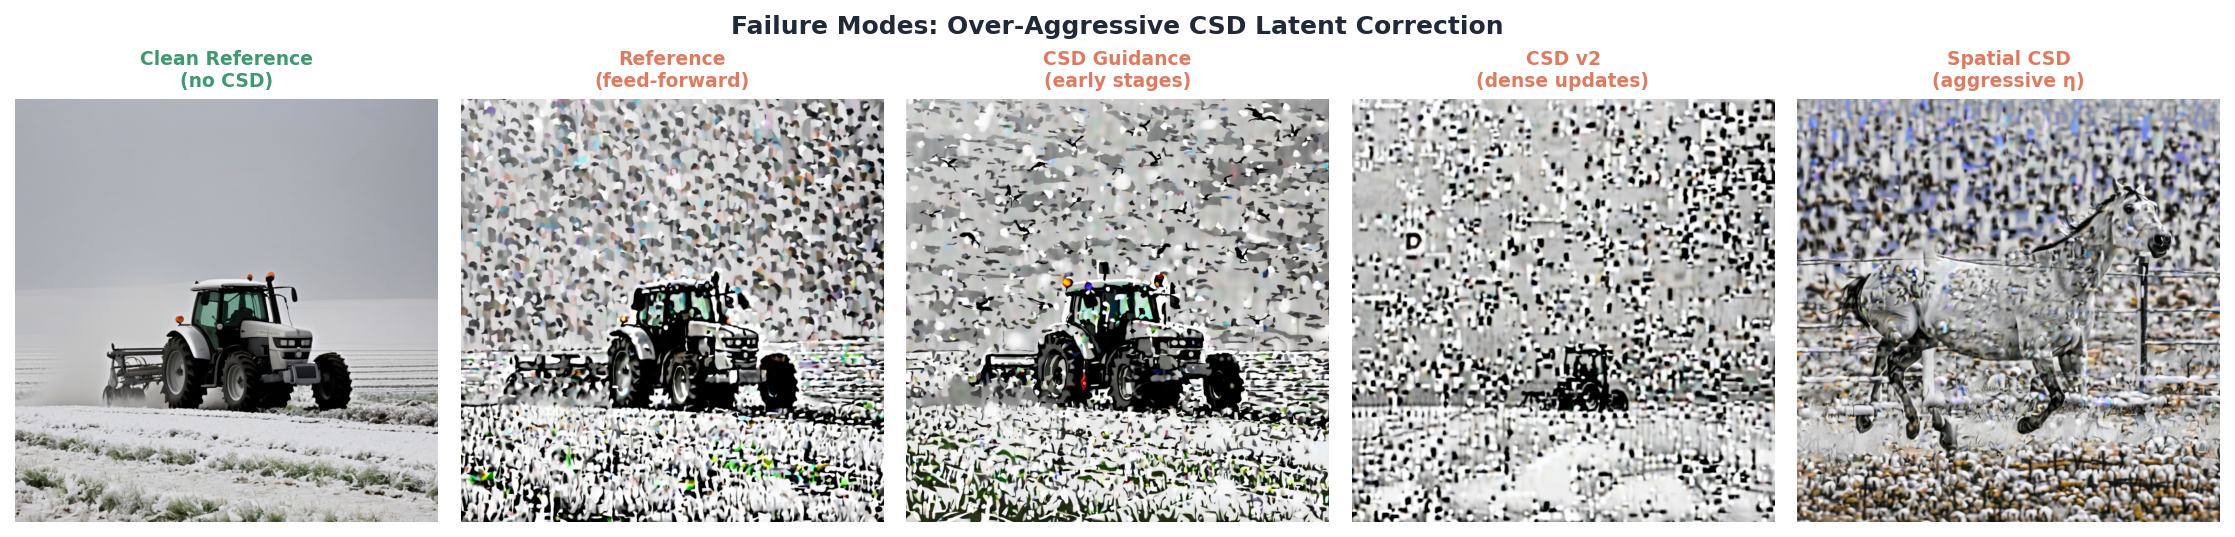
\includegraphics[width=0.95\linewidth]{images/ch7_langevin_failure.png}
    \caption{Typical failure cases observed in early Langevin-guided experiments. The aggressive optimization led to semantic collapse, structural distortions, and large-scale style leakage from the reference image.}
    \label{fig:ch7_langevin_failure}
\end{figure}

Further analysis showed that the performance of Langevin guidance is highly dependent on the stage in the diffusion process at which the optimization is applied. The overall semantic layout of the generated image is mostly decided by the early denoise steps. Therefore, strong style guidance at these stages often disrupts object formation and scene layout. In contrast, later denoising steps focus on refining appearance-level details and are thus a more suitable stage for optimizing atmospheric style.

In order to investigate this phenomenon, several optimization schedules were studied. The schedules differed in when they started the Langevin updates and how often they corrected during generation. Results consistently showed that the late-stage guidance led to better content preservation, while still making meaningful changes to the atmosphere.

Another important observation was the sensitivity of the optimization process to the selection of the learning rate. Small learning rates produced little stylistic change, while too large values destabilized generation and increased the chance of semantic collapse. It was found that a narrow intermediate range provided the best compromise between atmospheric realism and preservation of structure.

The main hyperparameters investigated in Langevin-guided diffusion experiments are summarized in Table~\ref{tab:langevin_hyperparameters}.

\begin{table}[htbp]
\centering
\caption{Hyperparameter configurations explored in Langevin-guided diffusion experiments.}
\label{tab:langevin_hyperparameters}
\renewcommand{\arraystretch}{1.3}
\begin{tabular}{lll}
\toprule
\textbf{Parameter} & \textbf{Values Explored} & \textbf{Observation} \\
\midrule
Learning rate & 0.001 -- 0.1 & Strength of style controlling \\
Optimization frequency & Sparse / Dense & Stability influence \\
Guidance Start Step & Early / Mid / Late & Impacts content preservation \\
Optimization Iterations & 1 -- 10 & Controls convergence \\
Noise Strength & Variable & Balances exploration \\
\bottomrule
\end{tabular}
\end{table}

Experiments also showed the limitations of unconstrained stochastic optimization, though Langevin refinement improved controllability over simple latent correction. The generated images were often inconsistent in their goals and it was still hard to find a stable trade-off between atmospheric style and semantic structure. These observations motivated the search for more principled optimization frameworks that can explicitly enforce constraints while preserving fidelity to the original diffusion trajectory.

We now consider Proximal Langevin Dynamics, which employs projection-based updates that constrain the latent corrections to feasible regions of the solution space. This formulation leads to a more stable mechanism for incorporating style constraints and ultimately forms the basis for the final optimization-driven framework investigated in this chapter.

\FloatBarrier
% =====================================================
\section{Proximal Langevin Dynamics}
\label{sec:ch7_pld}

The preceding section demonstrated that stochastic latent refinement can improve the atmospheric style match during diffusion sampling. However, unconstrained Langevin updates frequently introduced instability into the generation process. Strong optimization steps tended to cause latent trajectories to diverge from the natural diffusion manifold, resulting in semantic collapse, structural artifacts and over-reliance on the reference style image.

These observations illustrate a fundamental difficulty in optimization-guided diffusion. Stricter guidance generally leads to better style adherence at the cost of degrading image realism and content preservation. Therefore, a successful optimization framework needs to balance two conflicting objectives: preserving the fidelity to the learned diffusion prior, and satisfying the desired style constraints.

To overcome this limitation, the investigation turned to Proximal Langevin Dynamics (PLD), a constrained optimization framework that incorporates stochastic exploration and projection-based correction. Unlike the traditional Langevin update that directly updates the latent representations using the gradient information, PLD introduces an additional projection step to restrict the updates to a feasible region of the solution space.

The general proximal Langevin update can be written as:
\begin{equation}
    x_{t+1} = \mathrm{prox}_{\lambda g}\!\left( x_t + \gamma_t\,\nabla\log p(x_t) + \sqrt{2\gamma_t}\,\epsilon_t \right),
    \label{eq:proximal_loop}
\end{equation}
where $x_t$ is the current sample, $\gamma_t$ is the step size, $\epsilon_t$ is Gaussian noise, $g(\cdot)$ is the constraint function, and $\mathrm{prox}_{\lambda g}$ is the proximal operator.

The proximal operator acts as a projection mechanism that prevents the optimization from straying too far from areas that satisfy the desired constraints. PLD always maintains a balance between the diffusion objective and the constraint objective rather than allowing free latent updates. This results in a more stable optimization process.

\begin{figure}[htbp]
    \centering
    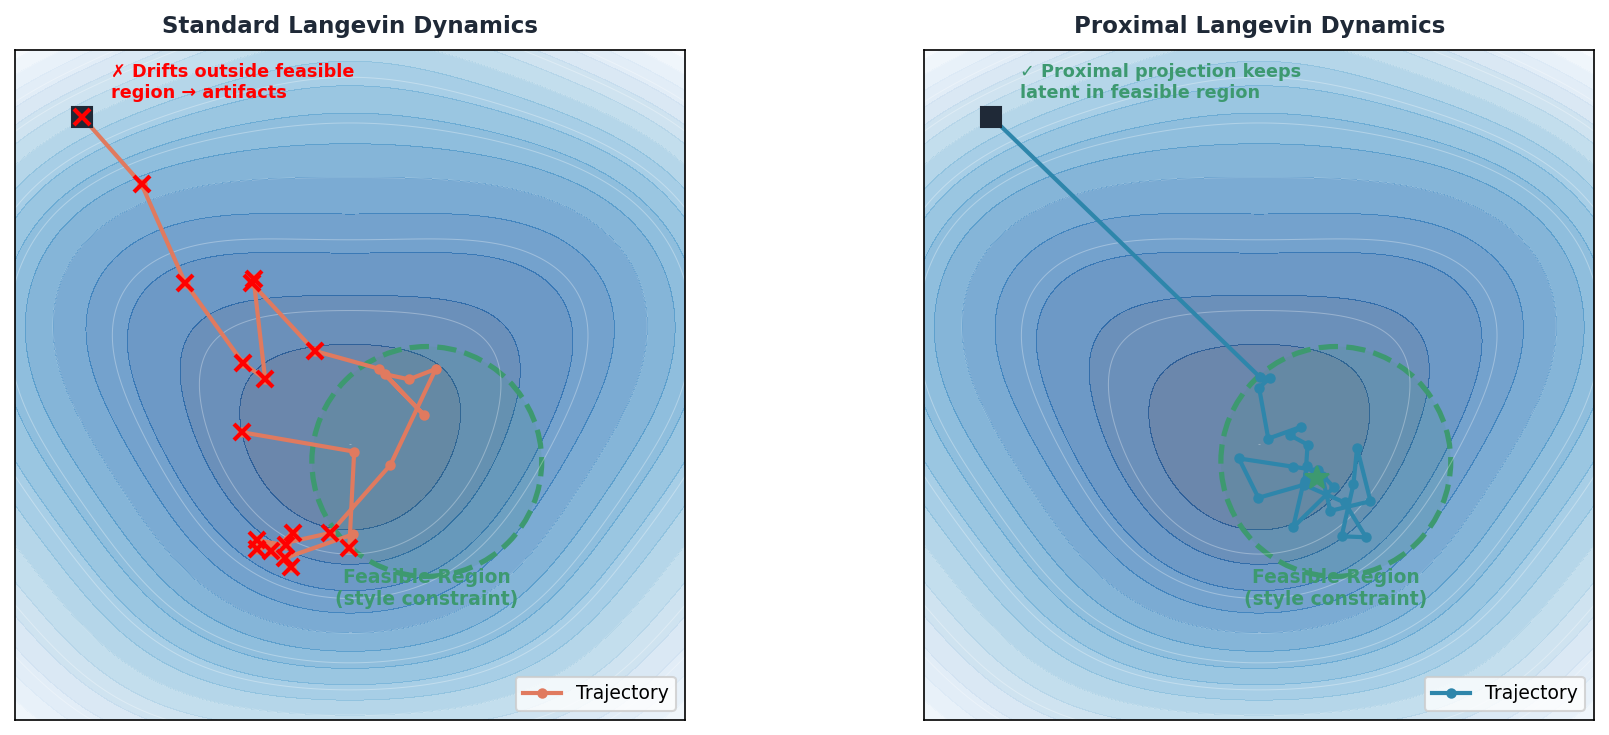
\includegraphics[width=0.95\linewidth]{images/ch7_pld_comparison.png}
    \caption{Unconstrained Langevin updates vs.\ Proximal Langevin Dynamics. The proximal operator restricts latent updates, preventing divergence from the diffusion manifold while enforcing the style constraint.}
    \label{fig:ch7_pld_comparison}
\end{figure}

In atmospheric style transfer, the proximal constraint was derived from style similarity objectives computed using CSD embeddings. The resulting image was decoded at selected time steps and compared to a reference image of atmospheric style. The calculated style loss was used to define a feasible region corresponding to acceptable atmospheric similarity.

This formulation has several advantages over standard latent correction. First, it reduces sensitivity to learning rate selection by bounding the magnitude of individual updates. Second, it reduces semantic collapse by avoiding large deviations from the prior diffusion. Third, it offers a principled way to incorporate multiple constraint functions into a unified optimization framework.

We could also include more sophisticated guidance objectives thanks to the use of proximal operators. Besides a simple cosine similarity, one could incorporate perceptual losses, feature-space statistics and frequency-domain constraints into the optimization procedure and still keep the generation behaviour stable.

Another advantage of PLD is that it is compatible with adaptive guidance schedules. The proximal formulation allows the strength of the guidance to adapt to the current denoising step, instead of a fixed optimization strength during the generation. This capability was found to be particularly useful for atmospheric style transfer, where different stages of the diffusion process play different roles in semantic structure and appearance formation.

The experimental results revealed that proximal Langevin updates consistently produced more stable results compared to standard Langevin refinement. The images exhibited better content preservation, less structural distortions, and smoother transitions to the target atmospheric style distribution. Although optimization was still computationally expensive, the increased stability of PLD made it the most promising optimization framework considered in this phase of the investigation.

The addition of proximal constraints also allowed us to explore richer style representations than the standard cosine similarity objectives. In particular, the atmospheric effects of fog, haze, snow and underwater images have specific frequency-domain properties that are not fully represented solely by embedding-space similarity. The next section therefore investigates how perceptual and frequency-aware constraints may be integrated into the optimization framework.

\begin{table}[htbp]
\centering
\caption{Comparison of latent correction, Langevin dynamics and proximal Langevin dynamics.}
\label{tab:optimization_comparison}
\renewcommand{\arraystretch}{1.3}
\begin{tabular}{lccc}
\toprule
\textbf{Method} & \textbf{Stability} & \textbf{Style Control} & \textbf{Content Preservation} \\
\midrule
Latent Correction & Medium & Medium & Medium \\
Langevin Dynamics & Low & High & Low \\
Proximal Langevin Dynamics & High & High & High \\
\bottomrule
\end{tabular}
\end{table}

\begin{figure}[htbp]
    \centering
    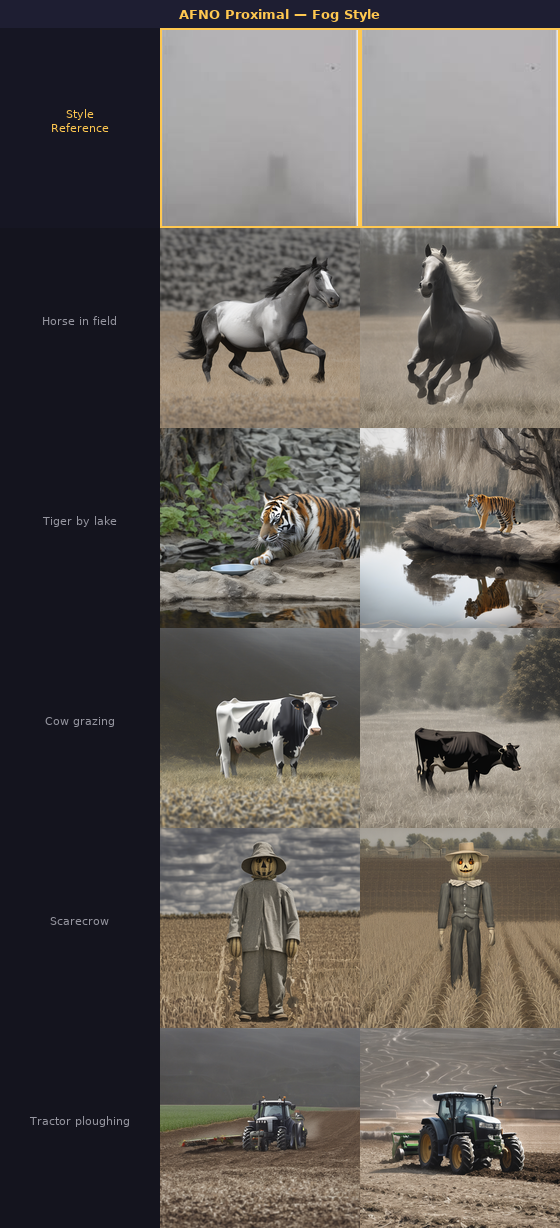
\includegraphics[width=0.6\linewidth, height=0.72\textheight, keepaspectratio]{images/ch7_grid_afno_proximal.png}
    \caption{Fog style transfer results using AFNO-based Proximal Langevin Dynamics (seed 42 and 123). The first row shows the fog style reference used as the optimisation target; subsequent rows show generated outputs per content prompt. The proximal projection operator constrains each latent update to the feasible region, yielding stable atmospheric transformations while preserving structural coherence.}
    \label{fig:ch7_afno_proximal}
\end{figure}

\FloatBarrier
% =====================================================
\section{Frequency-Based and Perceptual Constraints}
\label{sec:ch7_frequency}

The optimisation frameworks described in the previous sections are mostly based on style similarity computed in the CSD embedding space. These representations gave a semantically meaningful description of visual appearance, but empirical observations indicated that embedding similarity alone could not reliably capture atmospheric features.

Although the atmospheric behaviour was unrealistic, several generated images obtained high style similarity scores. In many cases the generated images were close to the reference style image in terms of overall colour distribution, but important atmospheric properties such as visibility degradation, contrast attenuation and depth-dependent scattering were still not well represented. These findings indicated that the semantic style embeddings fail to completely describe the atmospheric appearance.

Atmospheric phenomena are driven by physical image formation and global image statistics. Dense fog attenuates high-frequency image content, haze attenuates contrast as a function of depth, snowfall introduces structured texture patterns, and underwater environments generate wavelength-dependent colour attenuation. Thus, a guidance signal that relies solely on embedding similarity might fail to capture critical atmospheric features.

To address this limitation, the optimisation framework was augmented with additional perceptual and frequency-domain objectives. These objectives provide complementary information that is not explicitly available in the CSD embedding space, thereby offering a more complete description of atmospheric appearance.

\subsection{Perceptual Constraints}
\label{sec:ch7_perceptual}

Perceptual losses have become very popular in the areas of image synthesis and style transfer, since they compare images in a learned feature space instead of pixel-wise differences. Perceptual objectives operate on intermediate representations extracted from deep neural networks instead of directly measuring similarity in the image space.

Given a set of feature activations extracted from a pretrained encoder, the perceptual similarity can be expressed as:
\begin{equation}
    L_{\text{perc}} = \sum_{l} \bigl\|\phi_l(x_g) - \phi_l(x_s)\bigr\|_2^2,
\end{equation}
where $\phi_l(\cdot)$ is the activation of layer $l$, $x_g$ is the generated image and $x_s$ is the reference style image.

The main motivation for introducing perceptual guidance is the observation that atmospheric effects affect the structure of the image at a variety of scales. Local texture statistics, object boundaries, and global contrast relations all contribute to the perception of the environmental conditions. Such characteristics are captured by perceptual feature spaces, which therefore provide a richer representation of the atmospheric appearance than embedding similarity alone.

Experimental results showed that perceptual constraints improved content preservation and reduced a number of failure modes observed during cosine-only guidance. The generated images had more realistic atmospheric transitions and better preserved the structure of objects.

\subsection{Frequency-Domain Constraints}
\label{sec:ch7_freq}

Although perceptual guidance improved structural consistency, atmospheric phenomena have unique frequency-domain signatures not explicitly represented by feature-space objectives.

Fog, haze, smoke and underwater imagery are all associated with the attenuation of the high frequency image components. Increasing the atmospheric density suppresses fine details more and more, while the low frequency structures are relatively unaffected. Such behaviour can be seen directly in the Fourier spectrum of atmospheric images.

This observation motivated introducing constraints in the frequency domain through the Fourier Transform. The frequency representation of a generated image $x_g$ is calculated as:
\begin{equation}
    F_g = \mathcal{F}(x_g),
\end{equation}
where $\mathcal{F}(\cdot)$ is the two-dimensional Fourier Transform. The reference style image is represented as:
\begin{equation}
    F_s = \mathcal{F}(x_s).
\end{equation}

A frequency consistency objective can then be formulated as:
\begin{equation}
    L_{\text{freq}} = \bigl\| |F_g| - |F_s| \bigr\|_2^2,
\end{equation}
where $|F|$ is the magnitude spectrum.

The frequency loss promotes the generated images to share similar spectral characteristics of the target atmospheric domain. Unlike embedding-based objectives, this formulation imposes direct constraints on the distribution of image frequencies, providing a more physically meaningful description of visibility degradation.

\begin{figure}[htbp]
    \centering
    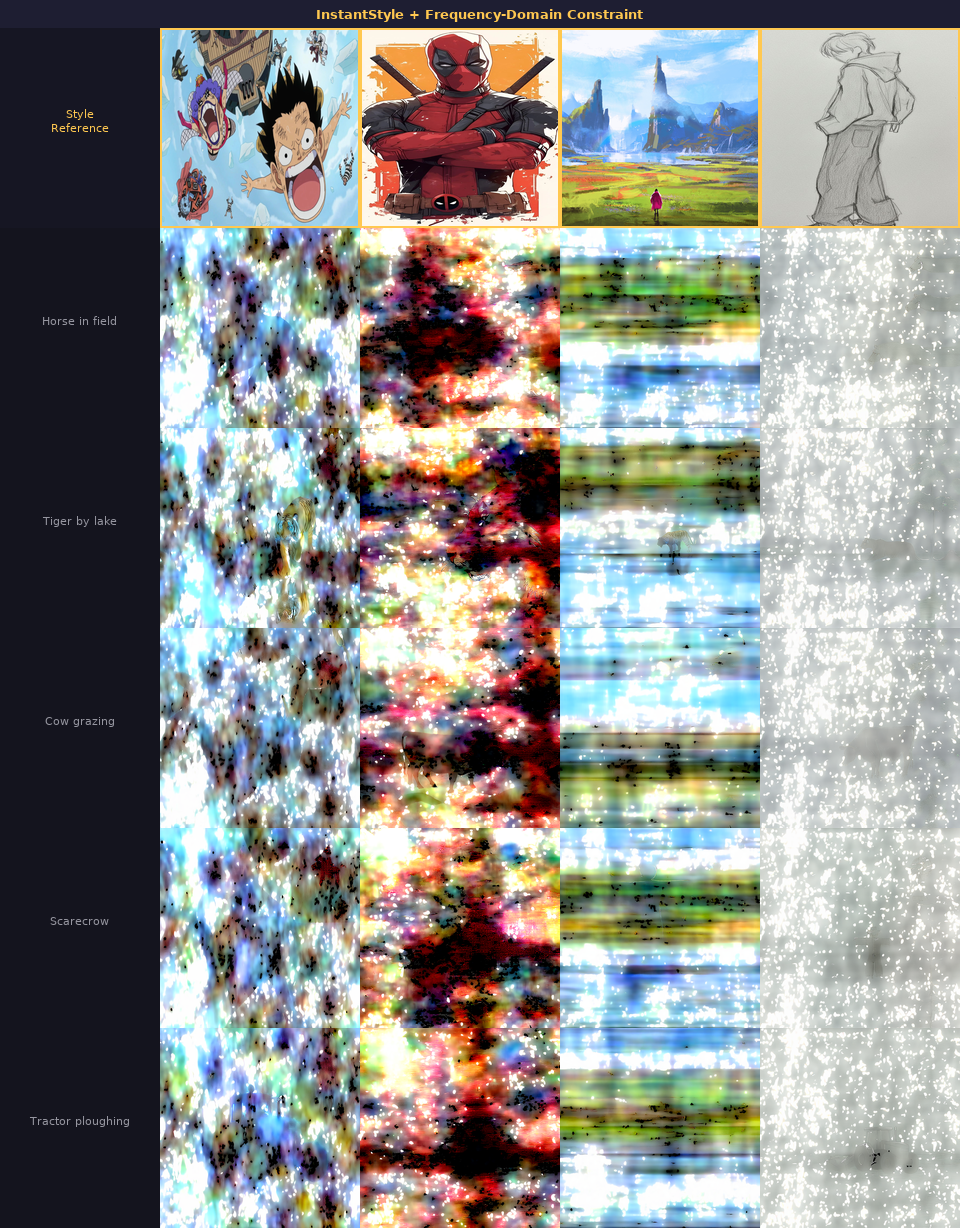
\includegraphics[width=0.88\linewidth, height=0.82\textheight, keepaspectratio]{images/ch7_grid_is_freq.png}
    \caption{InstantStyle + Frequency-domain constraint generation grid (seed 42). The first row shows the style reference image for each atmospheric domain; subsequent rows show generated outputs per content prompt. The FFT magnitude loss encourages the spectral envelope of each generated image to match the reference, producing more pronounced high-frequency attenuation characteristic of fog and sandstorm conditions.}
    \label{fig:ch7_grid_is_freq}
\end{figure}

\begin{figure}[htbp]
    \centering
    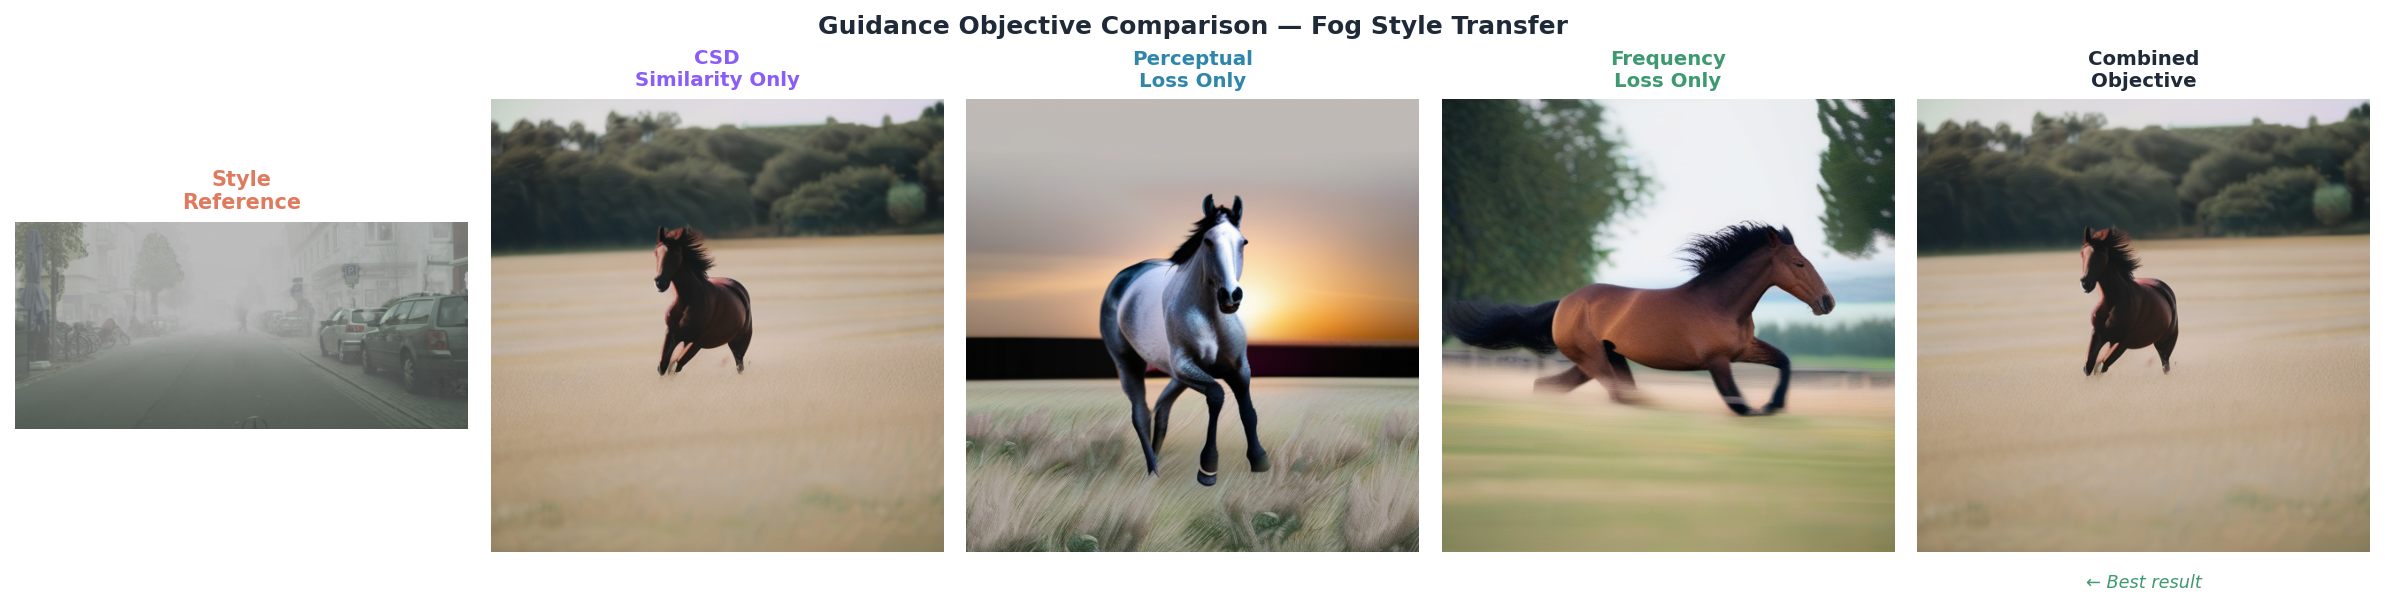
\includegraphics[width=0.95\linewidth]{images/ch7_objective_comparison.png}
    \caption{Comparison of different guidance objectives for atmospheric style transfer. The combined objective produces the most visually convincing results.}
    \label{fig:ch7_objective_comparison}
\end{figure}

\subsection{Combined Objective}
\label{sec:ch7_combined}

The final optimization framework consisted of multiple complementary objectives to capture different aspects of atmospheric appearance. The overall guidance objective is formulated as:
\begin{equation}
    L_{\text{total}} = \lambda_s\,L_{\text{style}} + \lambda_p\,L_{\text{perc}} + \lambda_f\,L_{\text{freq}},
\end{equation}
where $L_{\text{style}}$ is the CSD similarity loss, $L_{\text{perc}}$ is the perceptual guidance, and $L_{\text{freq}}$ is the frequency-domain consistency. The relative importance of each component is controlled by the weighting coefficients $\lambda_s$, $\lambda_p$ and $\lambda_f$.

Empirical evaluation showed that the joint objective always outperformed any individual loss term in producing more convincing atmospheric transformations. The style similarity guaranteed the semantic consistency with the reference image, the perceptual guidance preserved the structure of the scene, and the frequency constraints guided the realistic atmospheric degradation patterns. These objectives together provided a much richer representation of the atmospheric appearance, and laid the foundation for the final optimization-driven diffusion framework explored in this chapter.

\begin{table}[htbp]
\centering
\caption{Qualitative comparison of optimization objectives used in atmospheric style guidance experiments.}
\label{tab:objective_comparison}
\renewcommand{\arraystretch}{1.3}
\begin{tabular}{lccc}
\toprule
\textbf{Objective} & \textbf{Style Fidelity} & \textbf{Content Preservation} & \textbf{Stability} \\
\midrule
CSD Similarity & Medium & High & Medium \\
Perceptual Loss & Medium & High & High \\
Frequency Loss & High & Medium & Medium \\
Combined Objective & High & High & High \\
\bottomrule
\end{tabular}
\end{table}

\FloatBarrier
% =====================================================
\section{Experimental Progress and Discussion}
\label{sec:ch7_experiments}

The experiments described in this chapter were performed at different points in the development, each stage being prompted by observations from previous iterations. Instead of being developed from a fully optimization-guided framework from the start, the study was developed step-by-step through a series of experiments that aimed to understand the interaction between style constraints and diffusion-based image generation.

\subsection{Baseline Experiments: IP-Adapter on SDXL}
\label{sec:ch7_sd15}

Early experiments began with Stable Diffusion 1.5~\cite{rombach2022ldm}, confirming that direct CSD latent correction on the smaller backbone produced weak atmospheric effects and was highly sensitive to the learning rate. These results motivated a move to SDXL~\cite{podell2023sdxlimprovinglatentdiffusion}, whose richer latent representations and stronger generative prior offered a more stable foundation for optimization-based guidance.

The first SDXL experiments used IP-Adapter~\cite{ye2023ipadapter} as a feed-forward style conditioning baseline — no optimization guidance, just the adapter injecting style tokens into the cross-attention layers. Figure~\ref{fig:ch7_grid_ipadapter} shows the full generation grid across all tested style domains and content prompts. While the adapter transfers artistic styles (anime, comic, digital painting) convincingly, the atmospheric fog column is notably weak: generated images remain visually close to a clear-day scene, with no meaningful visibility degradation or haze formation. This confirms that feed-forward conditioning alone is insufficient for atmospheric style transfer and motivates the optimization-guided approaches explored throughout this chapter.

\begin{figure}[htbp]
    \centering
    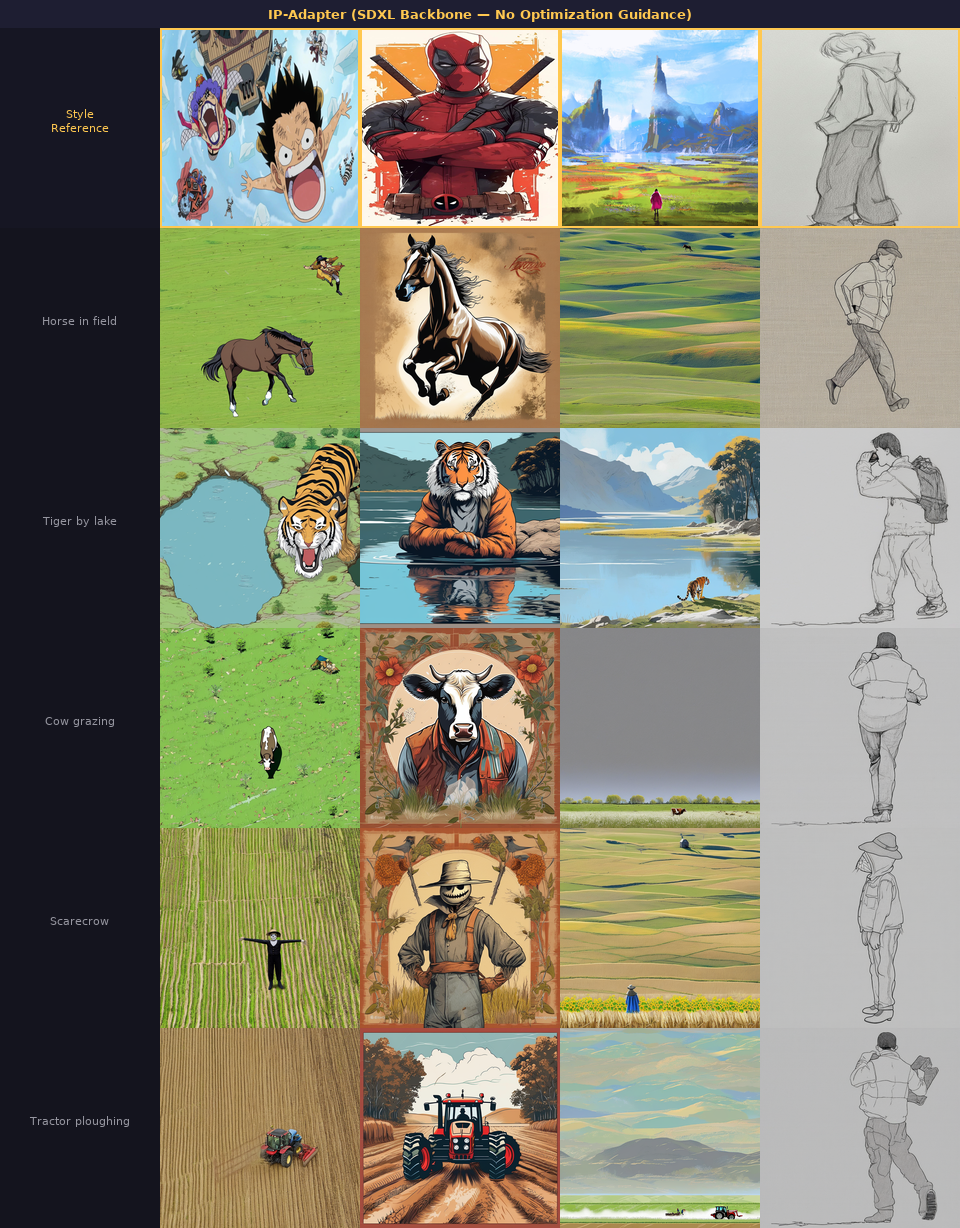
\includegraphics[width=0.95\linewidth]{images/ch7_grid_ipadapter.png}
    \caption{IP-Adapter (SDXL backbone) generation grid — seed 42. The first row in each style column shows the style reference image. Artistic styles (anime, comic, digital painting) transfer well; the fog\_style column produces clear-day images with negligible atmospheric effect, illustrating the limitation of feed-forward conditioning for atmospheric style transfer.}
    \label{fig:ch7_grid_ipadapter}
\end{figure}

\FloatBarrier
\subsection{Naive CSD Guidance and Its Failure Modes}
\label{sec:ch7_lora}

The natural next step was to augment IP-Adapter with CSD latent correction, applying gradient-based updates from the style loss throughout the denoising process. The expectation was that the optimization signal would bridge the gap the adapter could not close. In practice the opposite occurred: unconstrained CSD latent correction completely destabilised generation.

Figure~\ref{fig:ch7_grid_fog_failure} isolates the fog style domain to make the failure unambiguous: the IP-Adapter baseline (centre column) achieves plausible foggy scenes, confirming that the backbone and style injection work correctly. Adding unconstrained CSD latent correction (right column) collapses every single output into incoherent noise — the gradient signal overwhelms the diffusion prior and erases all semantic content. Figure~\ref{fig:ch7_grid_ipadapter_csd} shows that this collapse is not fog-specific; it occurs uniformly across all style domains and all content prompts. These failure modes reveal the core tension explored in the rest of this chapter: the style gradient must be introduced carefully, otherwise it destroys the very image structure it is meant to modify.

\begin{figure}[H]
    \centering
    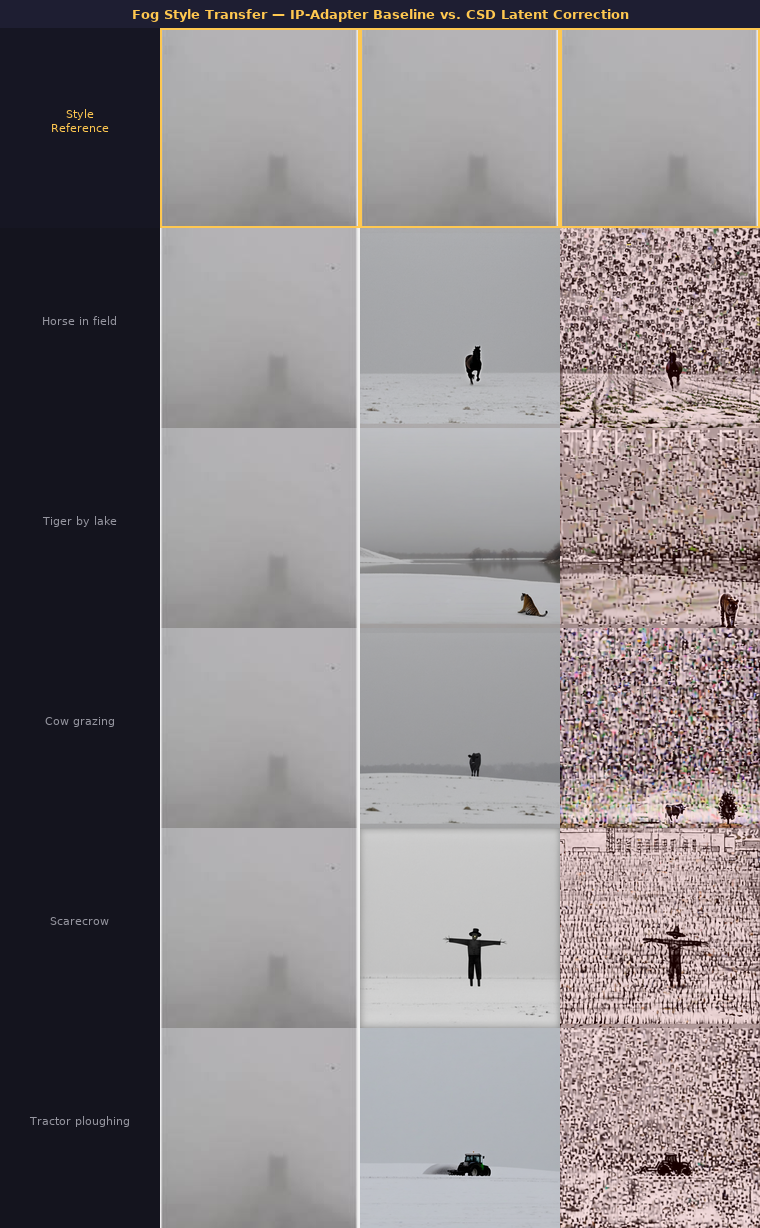
\includegraphics[width=0.44\linewidth]{images/ch7_grid_fog_failure.png}
    \caption{Fog-domain comparison (seed 42). \textbf{Centre column:} IP-Adapter alone produces plausible foggy scenes. \textbf{Right column (red tint):} adding unconstrained CSD latent correction destroys the image entirely, leaving tiled noise artefacts.}
    \label{fig:ch7_grid_fog_failure}
\end{figure}

\begin{figure}[htbp]
    \centering
    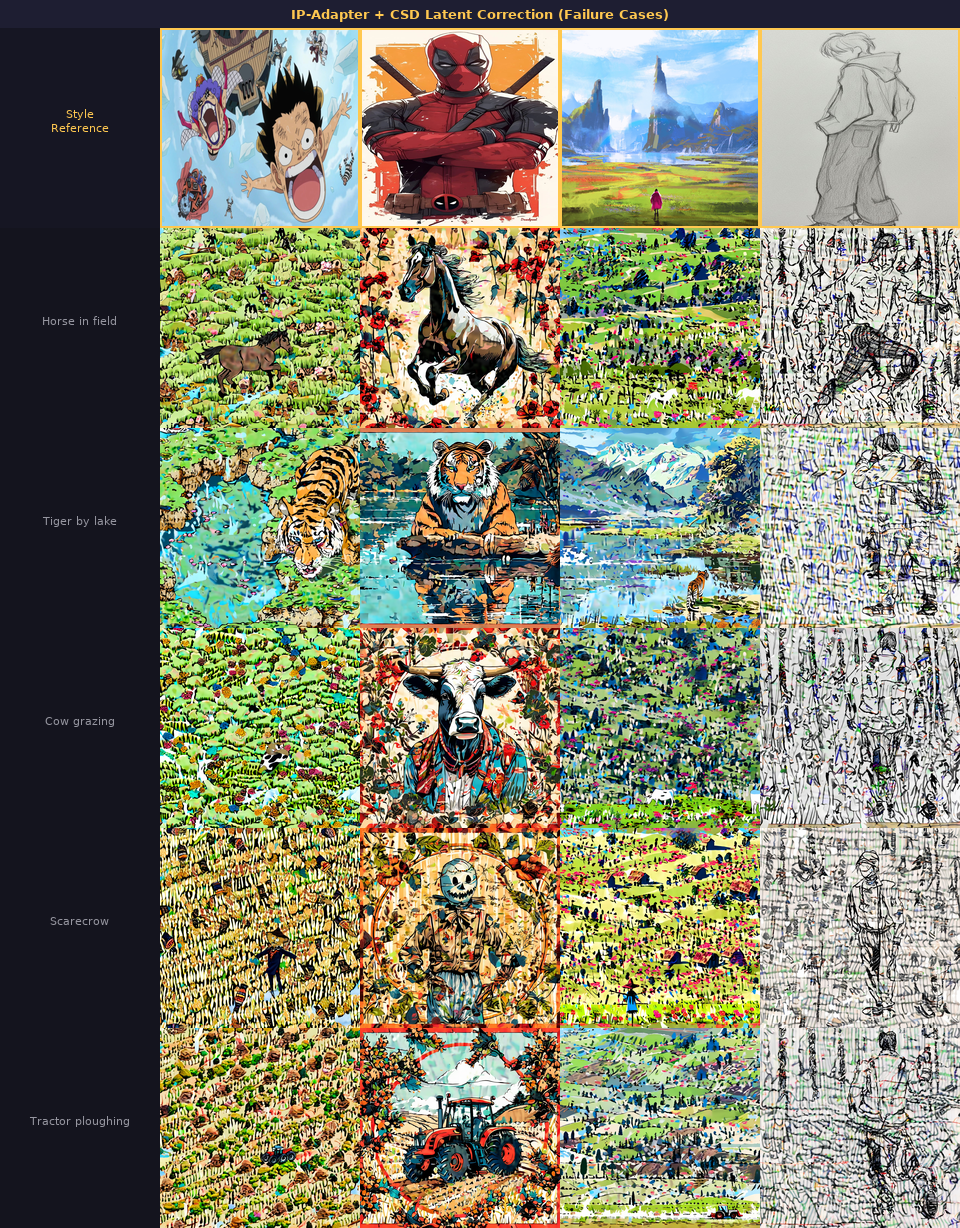
\includegraphics[width=0.88\linewidth, height=0.82\textheight, keepaspectratio]{images/ch7_grid_ipadapter_csd.png}
    \caption{IP-Adapter + unconstrained CSD latent correction across all style domains (seed 42). The first row shows the style reference for each domain. The collapse is universal — every prompt and every style produces incoherent tiled artefacts, confirming that the failure is a fundamental consequence of unconstrained latent correction rather than a style-specific issue. These failure modes directly motivate the constrained and stochastic optimisation strategies presented in Sections~\ref{sec:ch7_langevin}--\ref{sec:ch7_pld}.}
    \label{fig:ch7_grid_ipadapter_csd}
\end{figure}

\FloatBarrier
\subsection{Variable Guidance Schedules}
\label{sec:ch7_schedules}

One of the most important findings of the investigation was about the timing of optimization updates in denoising.

In early experiments, the style guidance was applied uniformly throughout the reverse diffusion process. This approach increased the style similarity, but often disturbed the formation of the semantic structure. Foreground objects were distorted, the scene composition degraded and the generated images sometimes collapsed towards the reference style image.

Later experiments used variable guidance schedules, where the strength of optimization was a function of the denoising progress. These schedules were motivated by the observation that early diffusion steps are mainly responsible for determining scene structure, while later steps refine appearance-level details.

The results consistently showed the superiority of late-stage guidance in terms of the trade-off between style fidelity and content preservation. In the last steps of the denoising process, strong optimization improved the atmospheric characteristics while preserving the semantic consistency.

\begin{figure}[htbp]
    \centering
    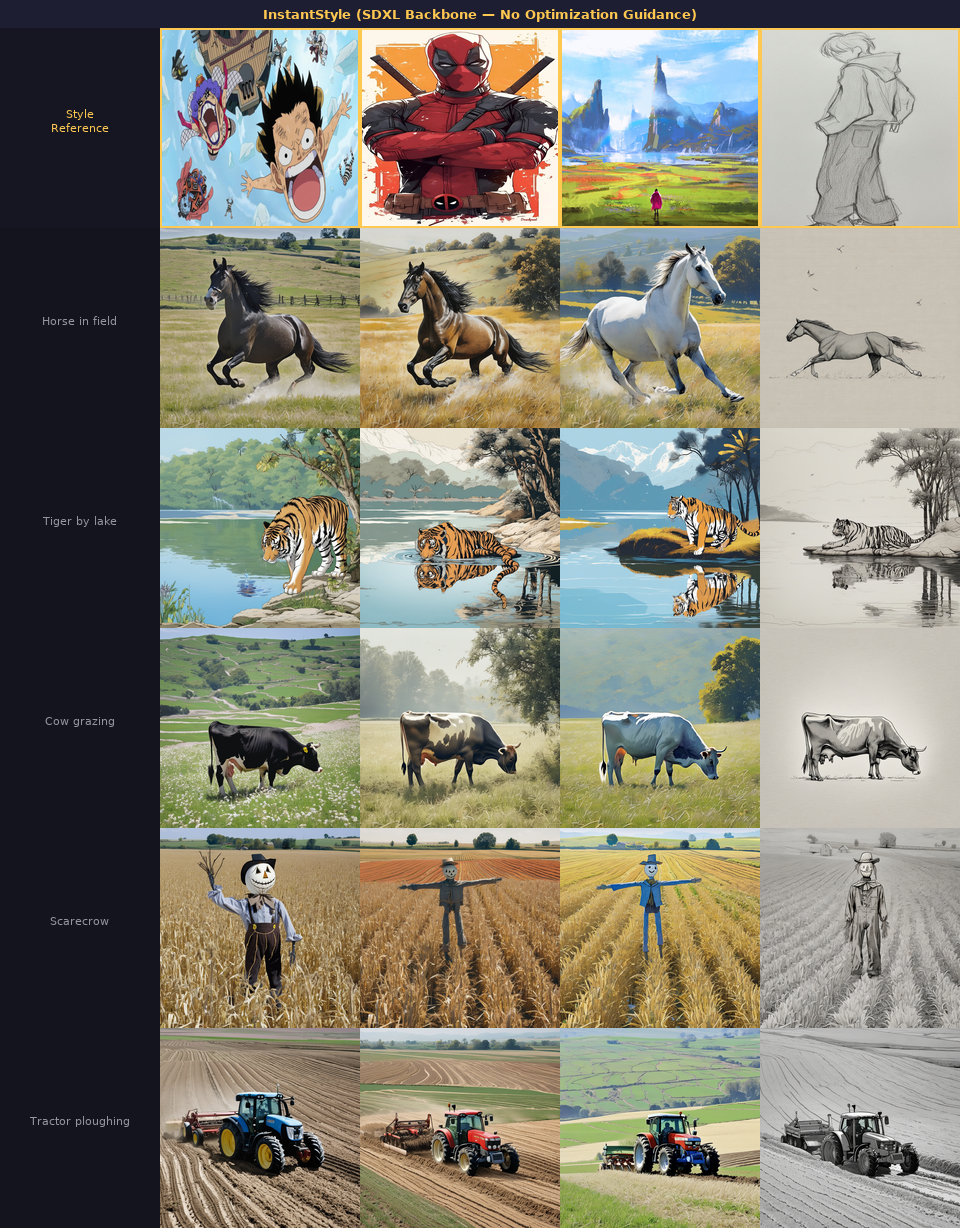
\includegraphics[width=0.95\linewidth]{images/ch7_grid_is_baseline.png}
    \caption{InstantStyle (SDXL backbone) clean feed-forward baseline grid — seed 42. The first row shows the style reference for each domain. This establishes the quality ceiling of the SDXL backbone with style injection but without any optimisation guidance; subsequent figures in this section should be read relative to this baseline.}
    \label{fig:ch7_grid_is_baseline}
\end{figure}

\begin{figure}[htbp]
    \centering
    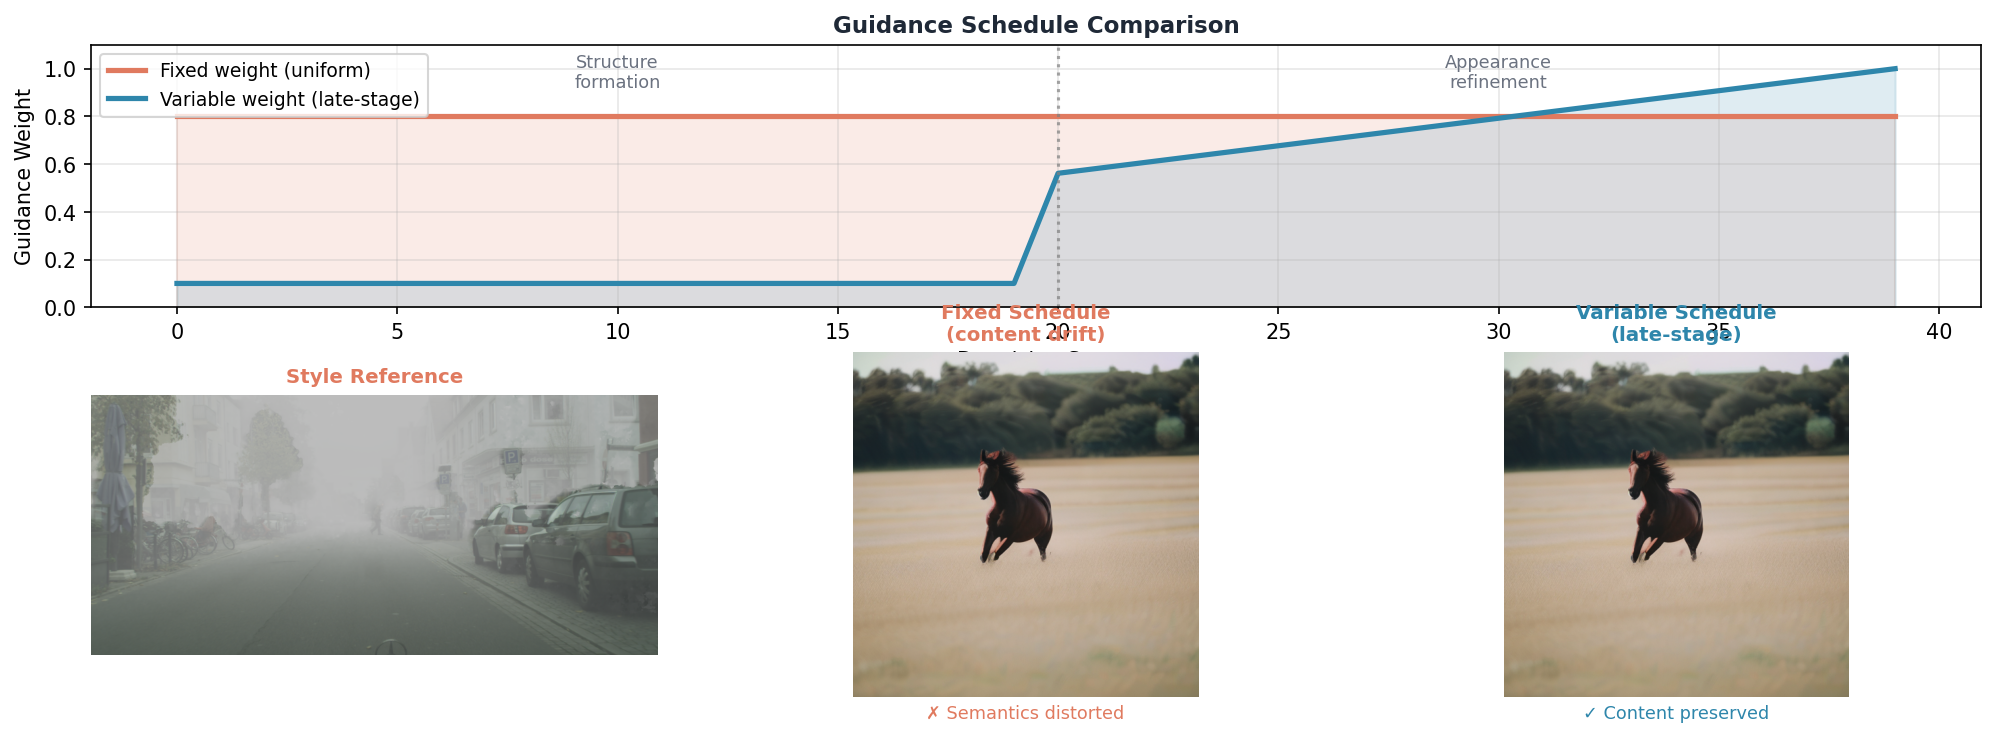
\includegraphics[width=0.95\linewidth]{images/ch7_fixed_vs_variable.png}
    \caption{Fixed versus variable guidance schedules. Late-stage optimization preserves the semantic content and allows for stronger atmospheric transformations.}
    \label{fig:fixed_vs_variable_weights}
\end{figure}

\FloatBarrier
\subsection{Case Studies: Fog Style Transfer}
\label{sec:ch7_casestudies}

To assess the developed framework on the target atmospheric domain, a focused evaluation on fog style transfer was conducted. Fog is a particularly challenging condition: it suppresses high-frequency information, degrades scene visibility, and requires depth-dependent contrast attenuation rather than a simple global colour shift. Optimisation-guided diffusion consistently generated more convincing fog effects than standard feed-forward conditioning, with the advantage most pronounced when frequency-domain constraints were included in the guidance objective.

\begin{figure}[htbp]
    \centering
    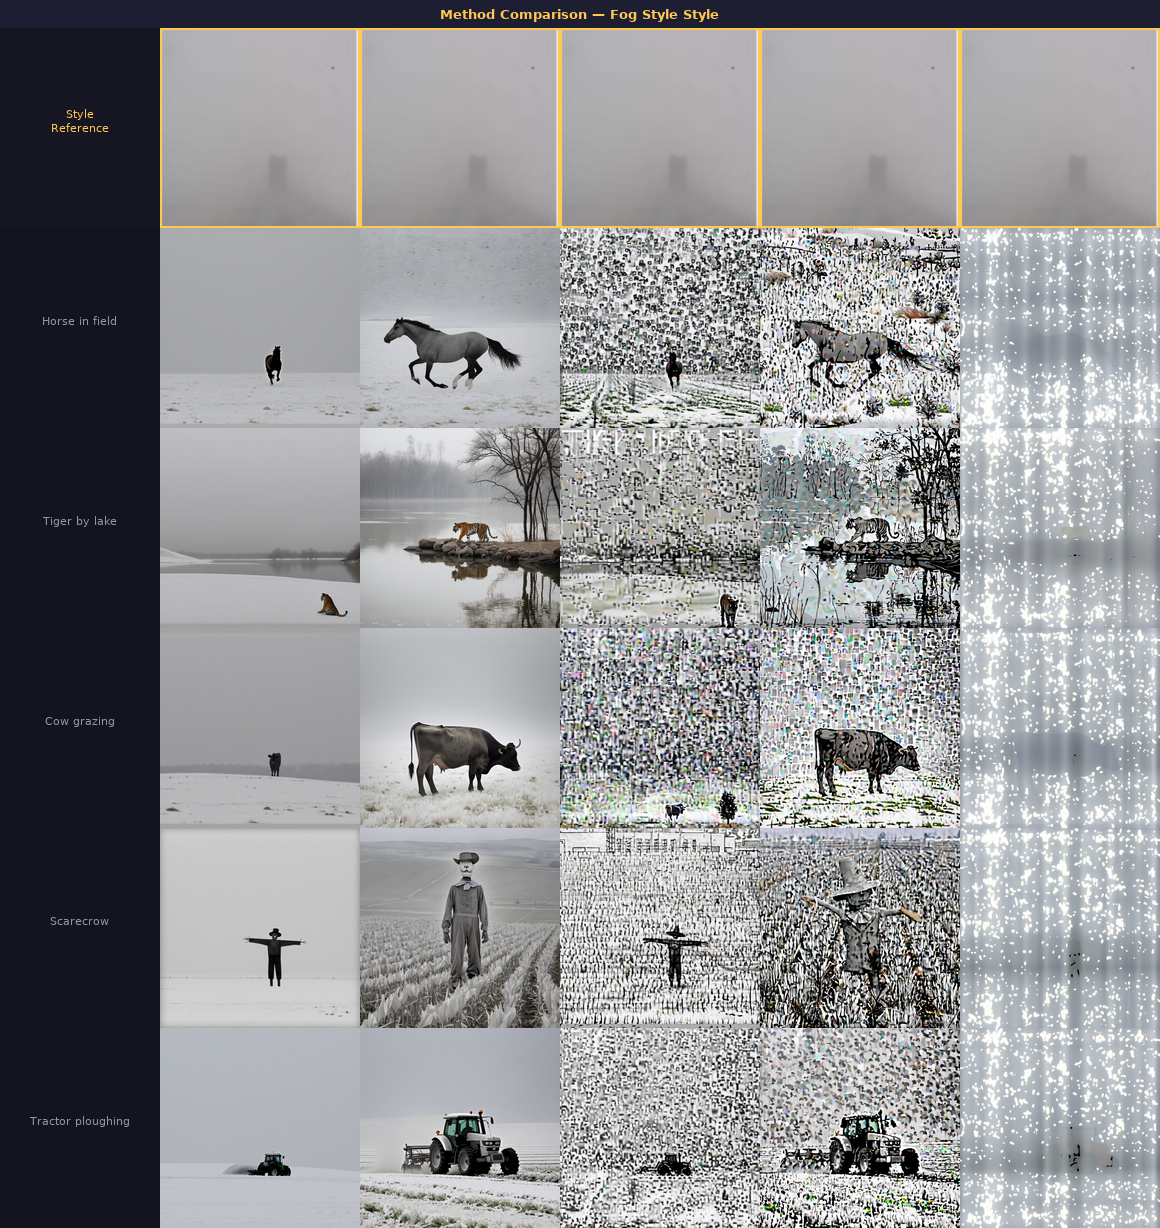
\includegraphics[width=0.95\linewidth]{images/ch7_grid_comparison.png}
    \caption{Multi-method comparison for fog atmospheric style transfer (seed 42). The first row shows the fog style reference image repeated across all method columns so the reader can judge each method against the same target; subsequent rows show generated outputs per content prompt. Columns compare IP-Adapter and InstantStyle baselines against their CSD and frequency-guided extensions, illustrating the trade-off between style fidelity and content preservation.}
    \label{fig:ch7_grid_comparison}
\end{figure}

\begin{figure}[htbp]
    \centering
    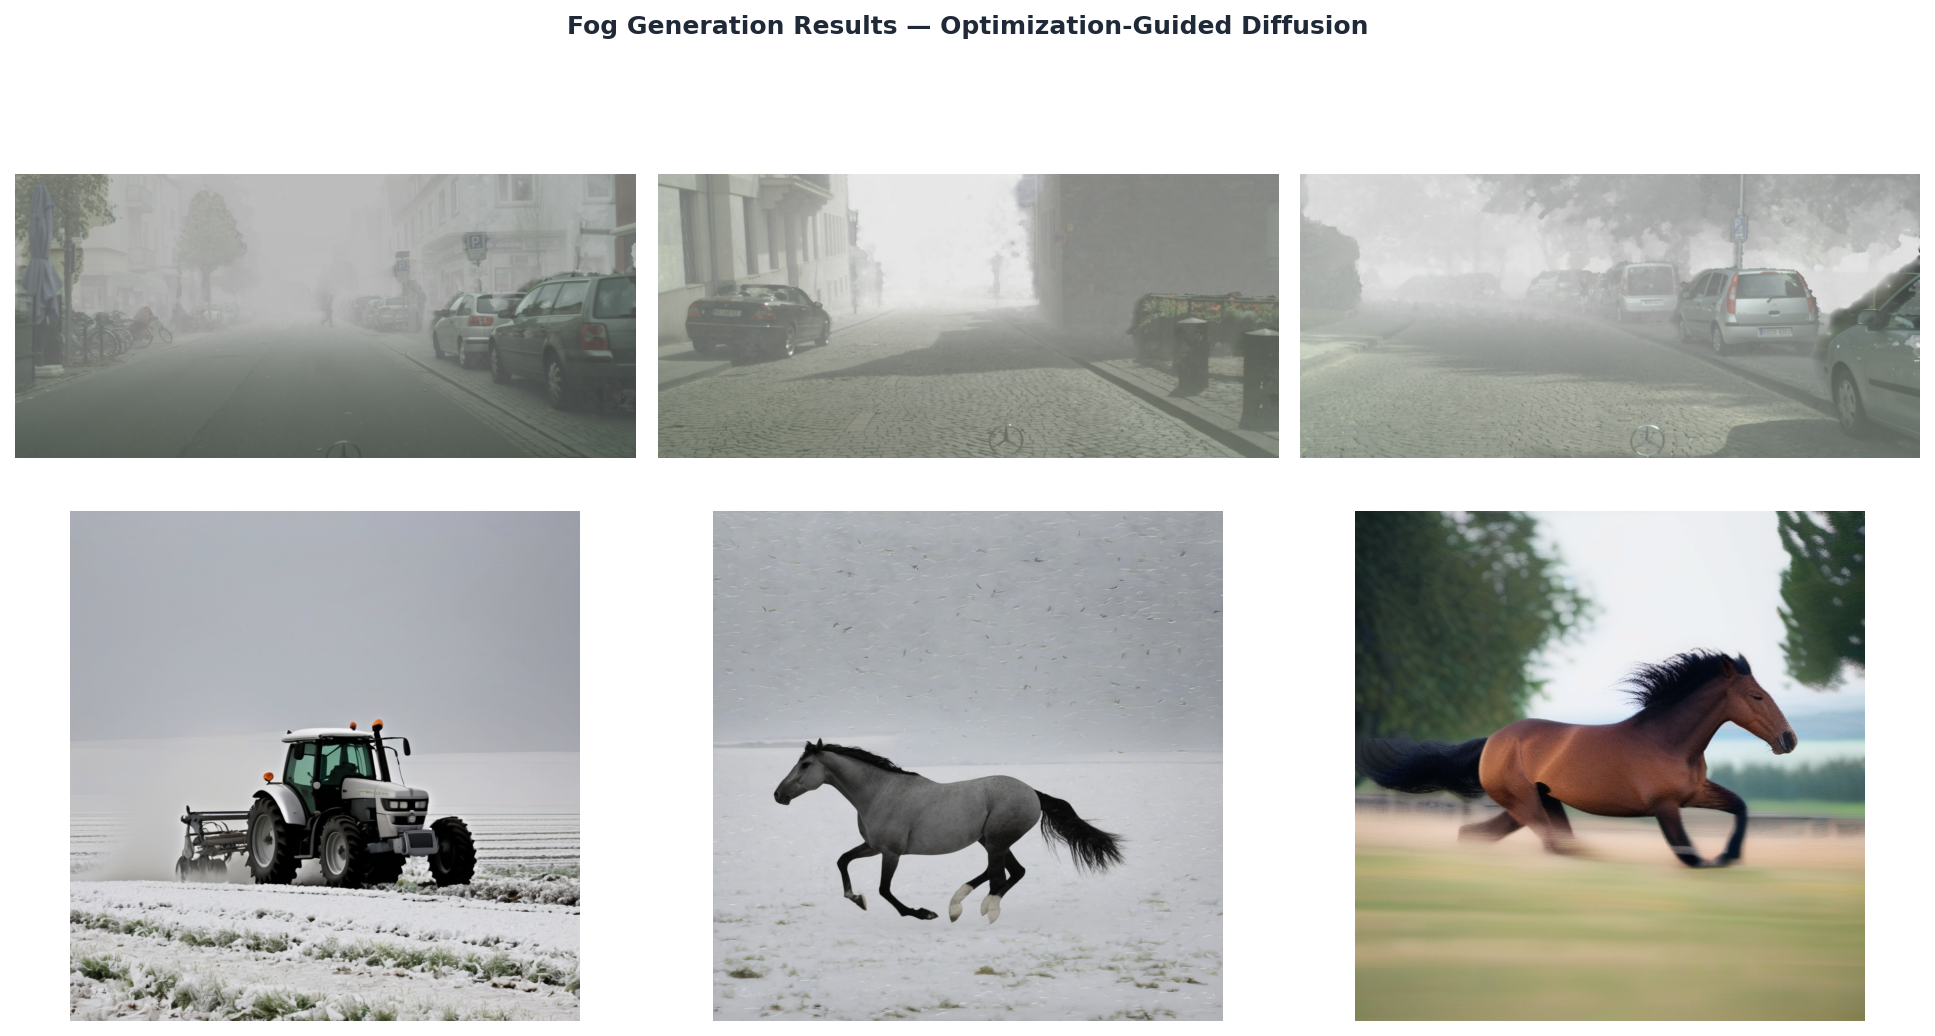
\includegraphics[width=0.95\linewidth]{images/ch7_fog_results.png}
    \caption{Representative results of fog generation via optimization-guided diffusion. Variable-weight schedule with frequency constraints produces realistic depth-dependent fog.}
    \label{fig:fog_style_results}
\end{figure}

\FloatBarrier
\subsection{Key Observations}
\label{sec:ch7_observations}

The experimental investigation yielded several important observations:

\begin{itemize}
    \item Style optimization is more effective when applied to later denoising steps.
    \item The atmospheric appearance is not representable with embedding-space similarity alone.
    \item Perceptual and frequency-domain constraints provide complementary information for better style fidelity.
    \item SDXL provides significant optimization stability improvements over Stable Diffusion 1.5.
    \item Unconstrained latent correction does not perform as well as proximal optimization strategies.
    \item Spectral guidance can be derived from the unique frequency characteristics of atmospheric phenomena.
\end{itemize}

These results collectively suggest that atmospheric style transfer can be framed as a constrained optimization problem in the reverse diffusion process. Further, they illustrate that good atmospheric guidance is obtained by combining semantic, perceptual and frequency-aware objectives, instead of depending on a single style representation.

\begin{table}[htbp]
\centering
\caption{Summary of key observations from the optimization-guided diffusion study.}
\label{tab:chapter7_findings}
\renewcommand{\arraystretch}{1.3}
\begin{tabular}{p{5.5cm} p{7.5cm}}
\toprule
\textbf{Observation} & \textbf{Consequence} \\
\midrule
Late-stage guidance is more effective & Changes atmospheric form while preserving semantic structure \\
SDXL $>$ SD1.5 & Better optimization stability with richer latent representations \\
Perceptual losses improve realism & Atmospheric effects beyond embedding similarity \\
Atmospheric phenomena have characteristic spectral signatures & FFT losses improve atmospheric fidelity \\
Proximal Langevin is more stable & Constrained optimization outperforms unconstrained updates \\
\bottomrule
\end{tabular}
\end{table}

\FloatBarrier
% =====================================================
\section{Summary}
\label{sec:ch7_summary}

This chapter explored optimisation-guided diffusion as an alternative atmospheric style transfer paradigm. Unlike traditional feed-forward style transfer methods that inject style information via conditioning mechanisms and rely solely on the diffusion model to interpret the given guidance, optimisation-guided diffusion introduces explicit objectives that are continuously enforced during the reverse diffusion process. This formulation transforms atmospheric style transfer from a passive conditioning problem into an active optimisation problem, where generated samples can be iteratively refined toward a target atmospheric distribution.

The investigation builds upon the constrained stable diffusion framework~\cite{zampini2025constrained}, which provides a generic mechanism for injecting user-specified objectives into the denoising process without modifying the diffusion model. Within this framework, Contrastive Style Descriptors (CSD)~\cite{somepalli2024csd} were studied as a style-aware representation for quantifying the atmospheric resemblance of generated images relative to style reference samples. Style losses computed on CSD embeddings were subsequently incorporated into the reverse diffusion process through latent-space optimisation.

Initial experiments showed that embedding-space guidance can successfully influence atmospheric appearance. However, the resulting optimisation process proved highly sensitive to hyperparameter selection and often exhibited unstable behaviour under strong guidance signals. These observations motivated the investigation of more principled optimisation strategies based on Langevin dynamics and Proximal Langevin dynamics. Stochastic latent refinement improved controllability and enabled stronger atmospheric transformations, but unconstrained updates frequently led to semantic degradation and reduced image quality. The introduction of proximal operators provided a more principled mechanism for balancing style adherence and fidelity to the diffusion prior, yielding substantially improved generation stability.

One important outcome of the investigation is that atmospheric appearance cannot be sufficiently described by embedding similarity alone. Global image statistics and frequency-domain properties govern atmospheric phenomena such as fog, haze, smoke, snowfall, and underwater environments in ways not captured by semantic style embeddings. This observation led to the integration of perceptual and frequency-aware objectives into the optimisation framework. Perceptual losses improved structural consistency and content preservation. Frequency-domain constraints provided a direct mechanism for modelling visibility degradation and the high-frequency attenuation characteristic of adverse environmental conditions.

The experimental progression produced several important findings. Optimisation-based guidance is far more effective when applied to later denoising steps, where appearance-level refinements dominate image formation. SDXL proved markedly more robust to optimisation-based interventions than Stable Diffusion 1.5, yielding enhanced image quality and more stable atmospheric transformations. Perceptual and spectral objectives consistently outperformed embedding-space similarity alone, confirming that atmospheric style is a fundamentally multi-faceted phenomenon requiring complementary representations. Constrained optimisation frameworks such as Proximal Langevin dynamics produced more reliable results than unconstrained latent correction strategies.

Although some experimental configurations did not yield stable results, the investigation produced valuable insights into the relationship between style representations, optimisation objectives, and diffusion-based image synthesis. The key conclusion is that atmospheric style transfer can be formulated as a constrained optimisation problem in the reverse diffusion process, and that explicit style objectives can guide generation without retraining the diffusion model.

These findings have direct implications for the physics-grounded synthesis framework presented in the following chapter. The limitations of purely embedding-based guidance and the importance of physically meaningful atmospheric representations motivated the development of a three-stage pipeline that combines depth estimation, atmospheric scattering models, and structured style injection to generate environmental transformations that are both visually convincing and physically consistent with real-world atmospheric phenomena.
